\documentclass[border=8pt]{standalone}
\usepackage{pgfplots}
\pgfplotsset{compat=1.18}
\begin{document}
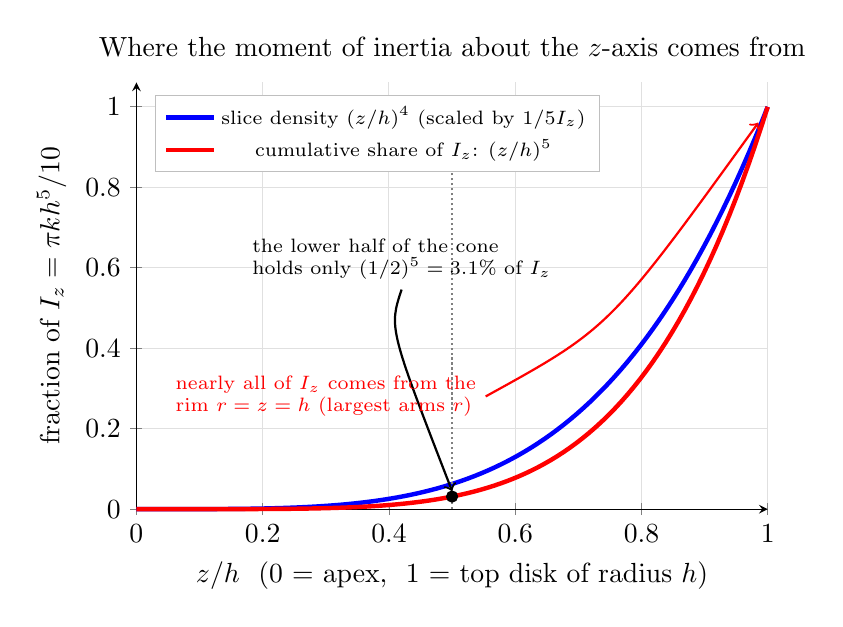
\begin{tikzpicture}
\begin{axis}[
  width=9.6cm, height=7.0cm,
  xlabel={$z/h$ \ (0 = apex,\ \ 1 = top disk of radius $h$)},
  ylabel={fraction of $I_z=\pi k h^5/10$},
  xmin=0,xmax=1, ymin=0,ymax=1.06,
  xtick={0,0.2,...,1}, ytick={0,0.2,...,1},
  grid=both, grid style={black!12},
  axis lines=left,
  title={Where the moment of inertia about the $z$-axis comes from},
  every title/.style={font=\small},
  legend style={at={(0.03,0.97)},anchor=north west,font=\scriptsize,fill=white,draw=black!25},
  clip=false]

  % shaded area under the slice-density curve (kept out of the legend)
  \addplot[blue!18, fill opacity=0.9, draw=none, domain=0:1, samples=100, forget plot] {x^4} \closedcycle;

  % slice density (scaled by 1/(5 I_z)) = (z/h)^4
  \addplot[blue, ultra thick, domain=0:1, samples=100] {x^4};
  \addlegendentry{slice density $(z/h)^4$ (scaled by $1/5I_z$)}

  % cumulative fraction = (z/h)^5
  \addplot[red, ultra thick, domain=0:1, samples=100] {x^5};
  \addlegendentry{cumulative share of $I_z$: $(z/h)^5$}

  \draw[gray, densely dotted, thick] (axis cs:0.5,0) -- (axis cs:0.5,0.95);
  \addplot[black, only marks, mark=*, forget plot] coordinates {(0.5,0.5^5)};
  \node[font=\scriptsize,black!60,right] at (axis cs:0.51,0.90) {$z=h/2$};

  \node[font=\scriptsize,align=left] (A) at (axis cs:0.42,0.62)
      {the lower half of the cone\\ holds only $(1/2)^5=3.1\%$ of $I_z$};
  \draw[black,thick,->] (A.south) .. controls (axis cs:0.40,0.45) .. (axis cs:0.50,0.045);

  \node[font=\scriptsize,red,align=left] (B) at (axis cs:0.30,0.28)
      {nearly all of $I_z$ comes from the\\ rim $r=z=h$ (largest arms $r$)};
  \draw[red,thick,->] (B.east) .. controls (axis cs:0.75,0.45) .. (axis cs:0.985,0.96);
\end{axis}
\end{tikzpicture}
\end{document}
